\documentclass[10pt,a4paper,landscape]{extarticle}
\usepackage[utf8]{inputenc}
\usepackage[T1]{fontenc}
\usepackage[ngerman]{babel}
\usepackage[a4paper,landscape,margin=0.6cm,columnsep=0.5cm]{geometry}
\usepackage{multicol}
\usepackage{amsmath,amssymb}
\usepackage{enumitem}
\usepackage{xcolor}
\usepackage{tcolorbox}
\usepackage{microtype}
\usepackage{array}
\usepackage{graphicx}

% --- Kompaktes Layout ---
\setlength{\parindent}{0pt}
\setlength{\parskip}{1.5pt}
\linespread{1.0}
\setlist{nosep,leftmargin=1.0em,topsep=0pt,partopsep=0pt,itemsep=0.4pt,parsep=0pt}
\setlist[itemize]{label=\textendash}
\pagestyle{empty}

% --- Farben ---
\definecolor{cA}{HTML}{1f4e79}
\definecolor{cB}{HTML}{1b6b2e}
\definecolor{cBox}{HTML}{eef3fa}
\definecolor{cFor}{HTML}{fff3df}
\definecolor{cWarn}{HTML}{fdeceb}
\definecolor{cEx}{HTML}{eaf5ea}

\newcommand{\sechead}[1]{\par\vspace{3pt}\noindent{\colorbox{cA}{\color{white}\bfseries\,#1\,}}\par\vspace{1.5pt}}
\newtcbox{\fbbox}{on line,boxrule=0.2pt,boxsep=1pt,left=2.5pt,right=2.5pt,top=1.2pt,bottom=1.2pt,colback=cFor,colframe=orange!55,arc=1pt}
\newcommand{\fb}[1]{\fbbox{\ensuremath{\displaystyle #1}}}
\newcommand{\K}[1]{\textbf{\color{cB}#1}}
\newcommand{\R}[1]{\textbf{\color{red!72!black}#1}}
\newtcolorbox{exbox}{colback=cEx,colframe=cB!70!black,boxrule=0.3pt,left=2.5pt,right=2.5pt,top=1.5pt,bottom=1.5pt,arc=1pt,before skip=2pt,after skip=2pt}

\begin{document}
\small
\begin{multicols}{5}

\sechead{Bilanz (Bestandesrechnung)}
\K{Aktiven} (Mittelverwendung – ``worin angelegt''):
\begin{itemize}
\item \K{Umlaufverm.\ (UV)}: flüssig oder Umwandlung $<$1\,J
— Kasse, Post, Bank, Ford.\ L+L, Vorräte, Aktive Rechnungsabgrenzungen (ARA).
\item \K{Anlageverm.\ (AV)}: Nutzung $>$1\,J
— Mobilien, Immobilien, Beteiligungen, Patente.
\end{itemize}
\K{Passiven} (Mittelherkunft – ``wer gab Kapital''):
\begin{itemize}
\item \K{FK kurzfr.} ($<$1\,J): Verb.\ L+L, Kundenanzahlungen, PRA.
\item \K{FK langfr.} ($>$1\,J): Darlehen, Hypothek, Rückstellungen.
\item \K{EK}: Aktienkapital, Reserven, Gewinnvortrag, Jahresgewinn.
\end{itemize}
\fb{\text{Summe Aktiven}=\text{Summe Passiven}}\\
\fb{EK=\text{Aktiven}-FK}\\
Liquidität: UV von oben nach unten zunehmend gebunden.

{\centering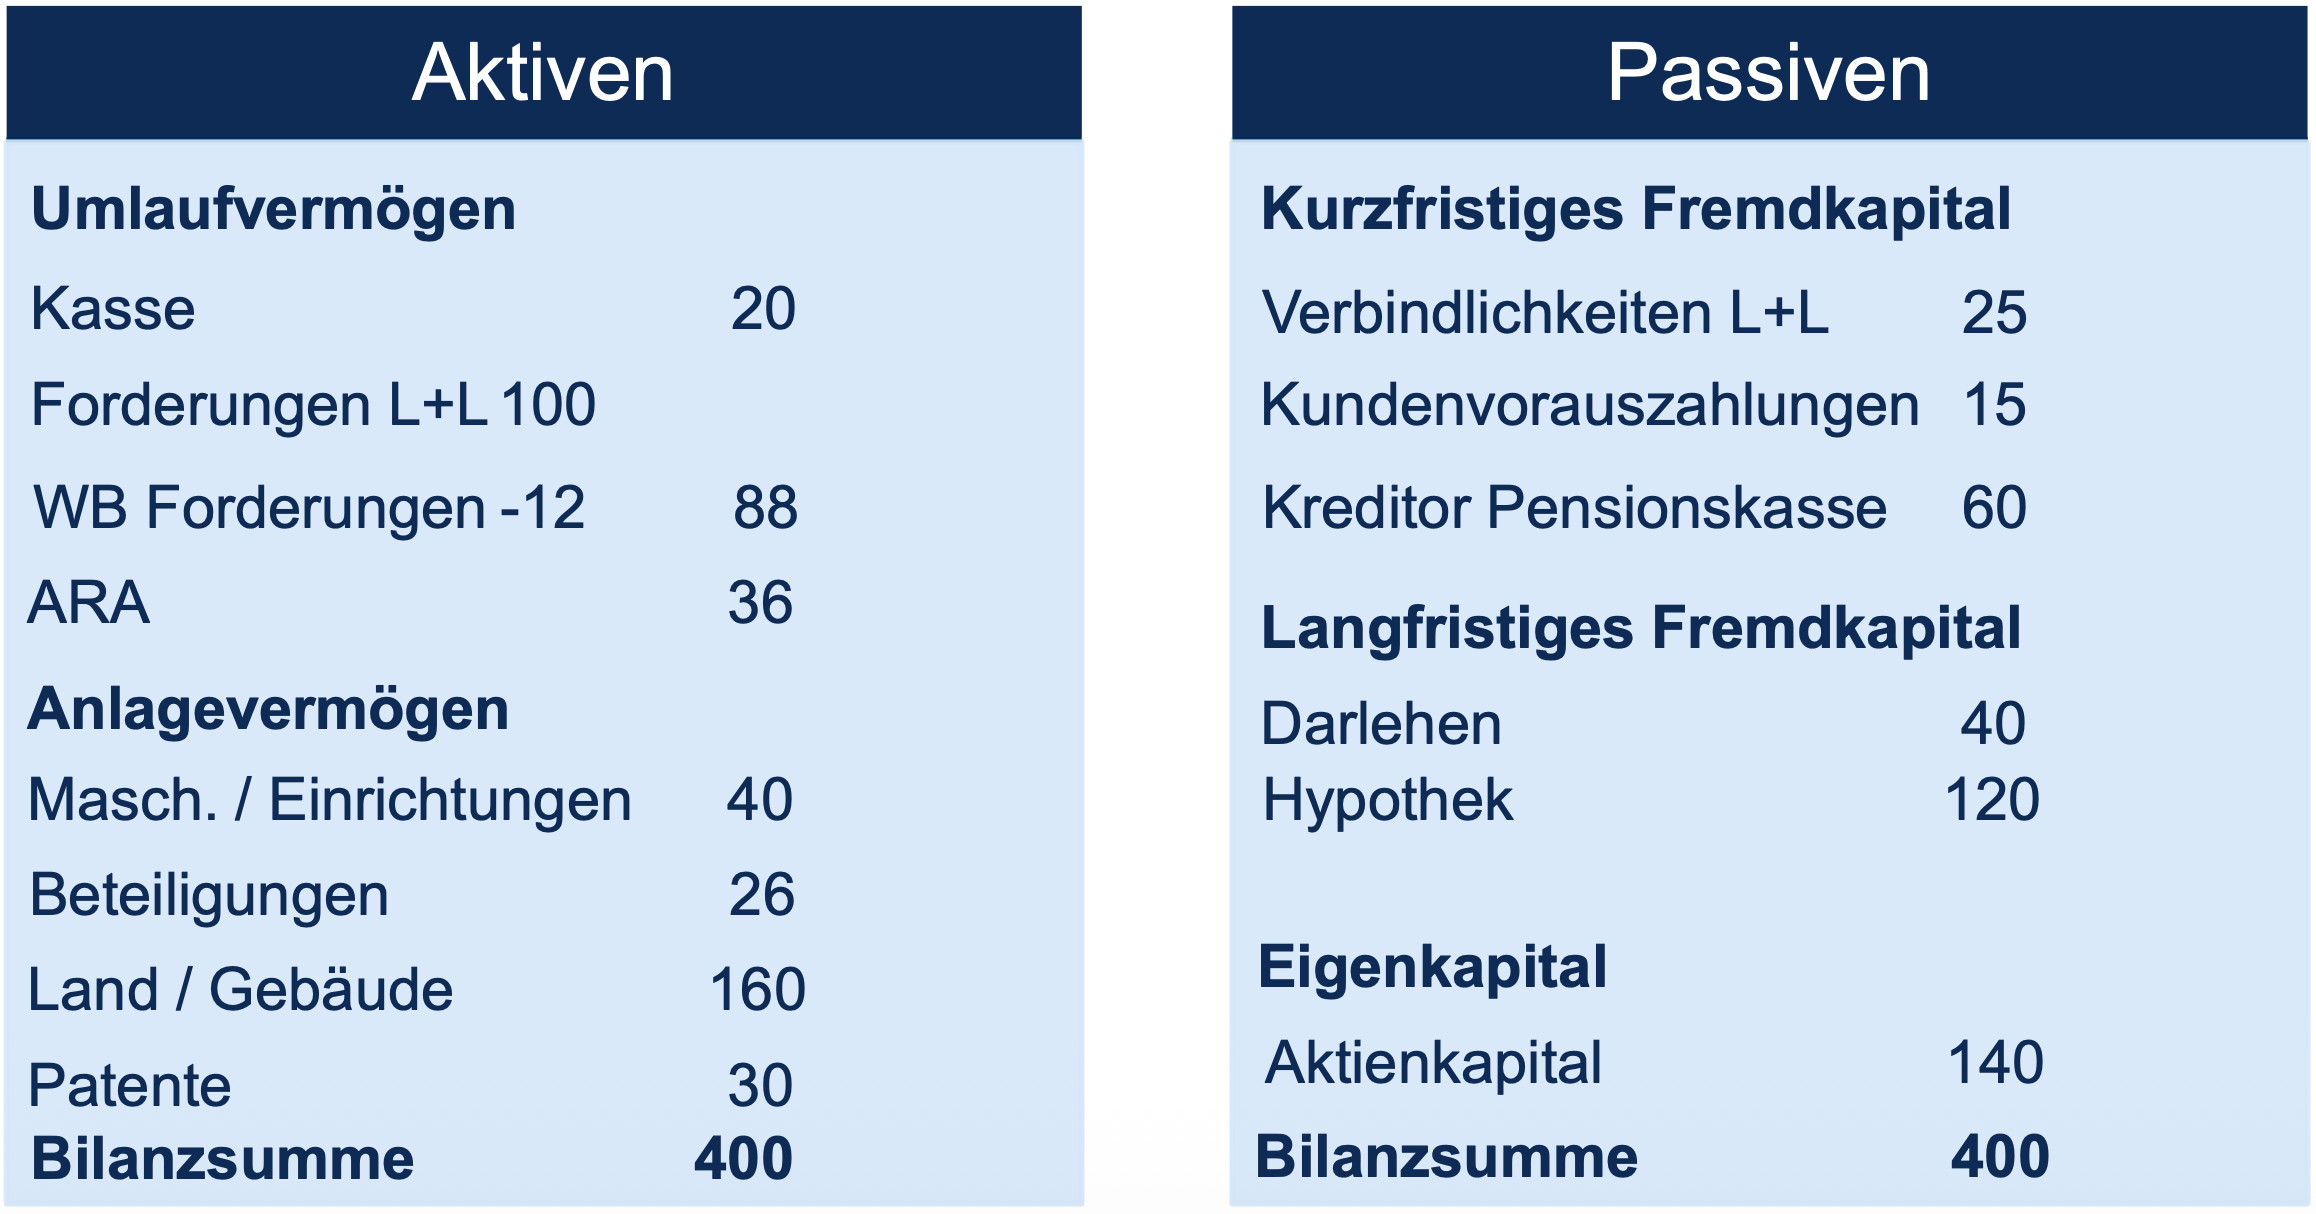
\includegraphics[width=\linewidth]{imgages/bilanz.png}\par}

\begin{exbox}
\textbf{Kennzahlen}\\
EK-Quote $=\tfrac{EK}{GK}$; Verschuldungsgrad $=\tfrac{FK}{GK}$\\
GK-Rendite $=\tfrac{\text{Gewinn}+\text{FK-Zins}}{GK}$\\
EK-Rendite $=\tfrac{\text{Gewinn}}{EK}$ (Leverage, wenn GK-Rendite $>$ FK-Zins)\\
Liquiditätsgrade: flüssige Mittel bzw.\ UV im Verhältnis zu kurzfr.\ FK.
\end{exbox}

\sechead{Erfolgsrechnung (mehrstufig)}
Stellt Aufwand \& Ertrag einer Periode gegenüber
$\Rightarrow$ Gewinn (Ertrag$>$Aufwand) oder Verlust.\\
\begin{tabular}{@{}r@{~}l@{}}
 & Betrieblicher Ertrag (aus L+L)\\
$-$ & Waren-/Materialaufwand\\
$=$ & \textbf{Bruttoergebnis}\\
$-$ & Personalaufwand\\
$-$ & übrige Aufwände (Miete, Werbung,\\
 & Unterhalt, Kommunikation, Abgaben)\\
$=$ & \K{EBITDA}\\
$-$ & Abschreibungen\\
$=$ & \K{EBIT} (Betriebsgewinn)\\
$-$ & Zinsaufwand (Finanzaufwand)\\
$=$ & \K{EBT} (Gewinn vor Steuern)\\
$-$ & Steueraufwand\\
$=$ & \K{Reingewinn / Jahresgewinn}\\
\end{tabular}

{\centering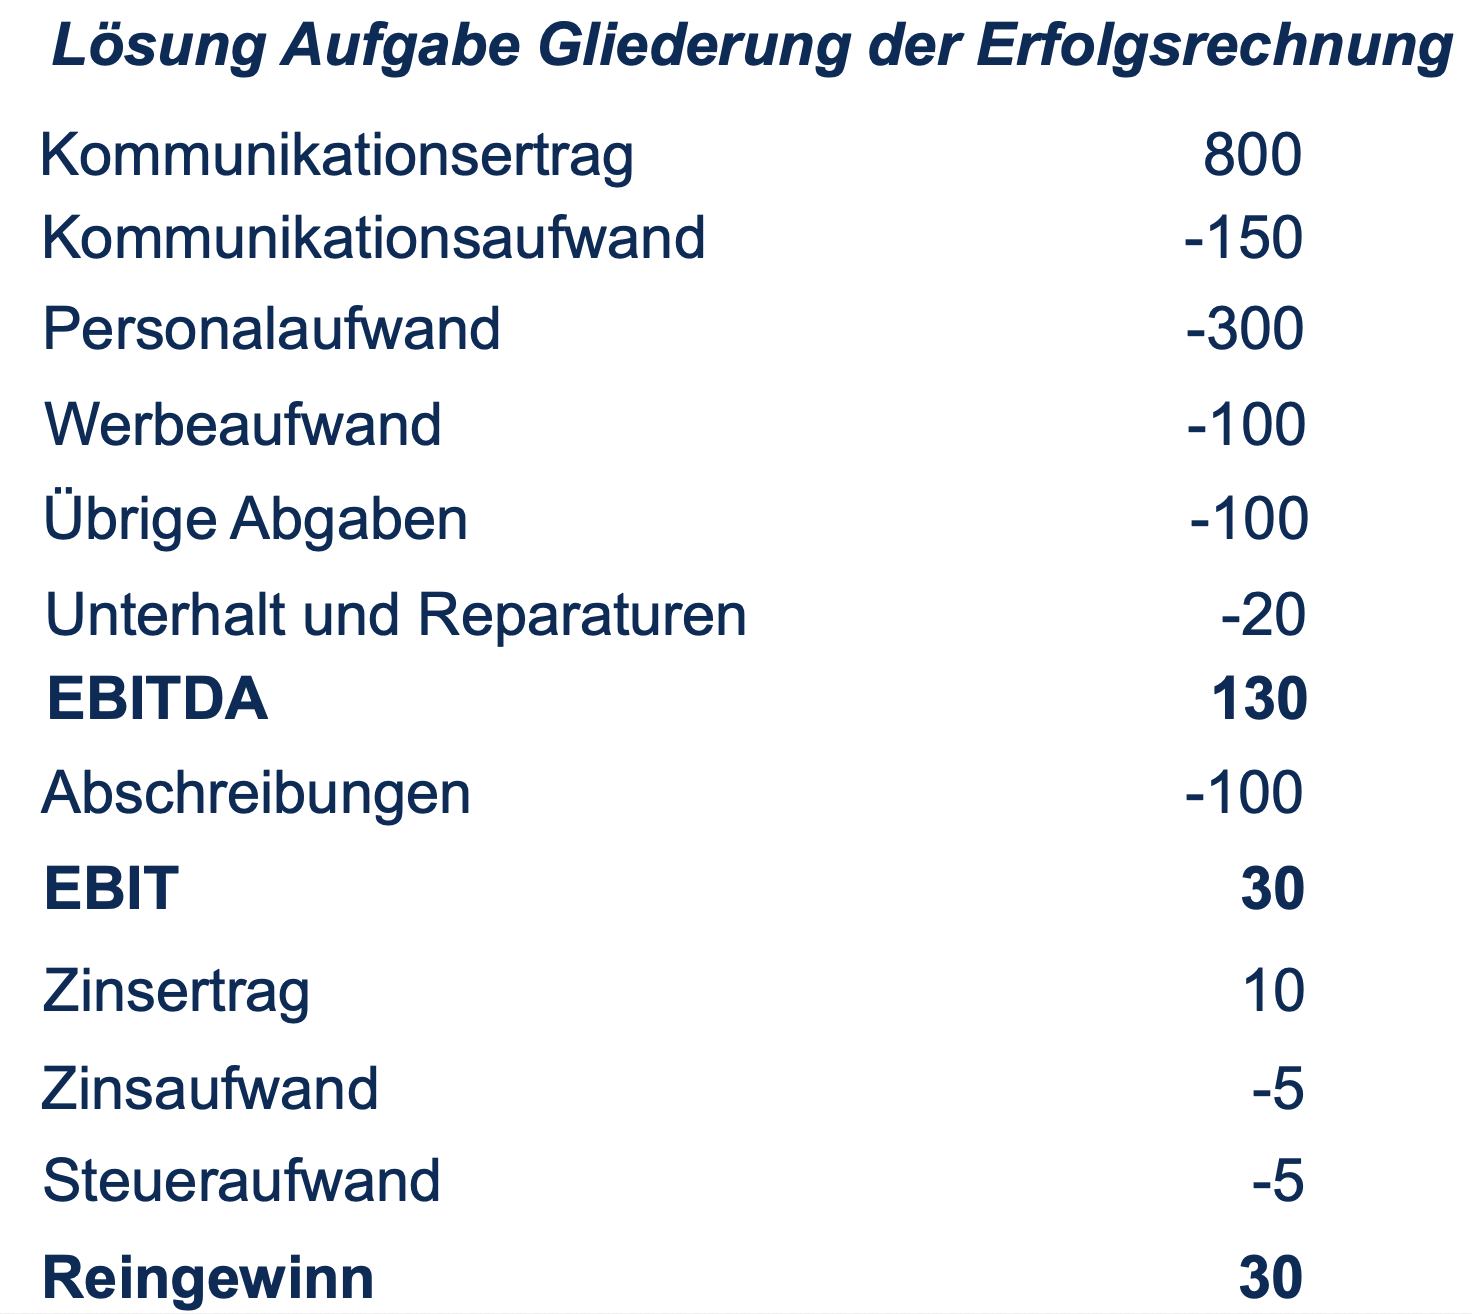
\includegraphics[width=\linewidth]{imgages/erfolgsrechnung.png}\par}

\begin{exbox}
\textbf{Tuti AG} (CHF): Ertrag 600'000;
Personal 300'000;
Miete 60'000;
Abschr.\ 30'000;
Zins 30'000;
Steuer 40'000.\\
EBITDA $=600{-}300{-}60=\R{240'000}$\\
EBIT $=240{-}30=\R{210'000}$\\
EBT $=210{-}30=180'000$\\
Reingewinn $=180{-}40=\R{140'000}$\\
\footnotesize Zins \& Steuer sind \emph{kein} Betriebsaufwand
$\Rightarrow$ erst nach EBIT.
\end{exbox}

\sechead{Geldflussrechnung (Cashflow)}
Zeigt die Fähigkeit, Zahlungsmittel zu erwirtschaften, \& den Bedarf.\\
\K{Ertrag/Aufwand $\neq$ Ein-/Auszahlung}: eine Ein-/Auszahlung ist \emph{immer} Geldfluss;
Abschreibung \& Bildung Rückstellung sind Aufwand \emph{ohne} Geldfluss (nicht liquiditätswirksam).
Wertzunahme Wertschrift = Ertrag ohne Einzahlung.\\
\K{3 Bereiche:} CFO (Betrieb),
CFI (Investition: Kauf $-$ / Verkauf $+$ Anlagen),
CFF (Finanzierung: Aufnahme $+$ / Rückzahlung $-$ FK \& EK).
Summe $=$ Veränderung flüssige Mittel.\\
\K{Direkt}: liq.-wirksame Erträge $-$ liq.-wirksame Aufwände, je über Gegenkonto
(z.B.\ Warenertrag $-$ Zunahme Ford.\ L+L $=$ Zahlung Kunden).\\

{\centering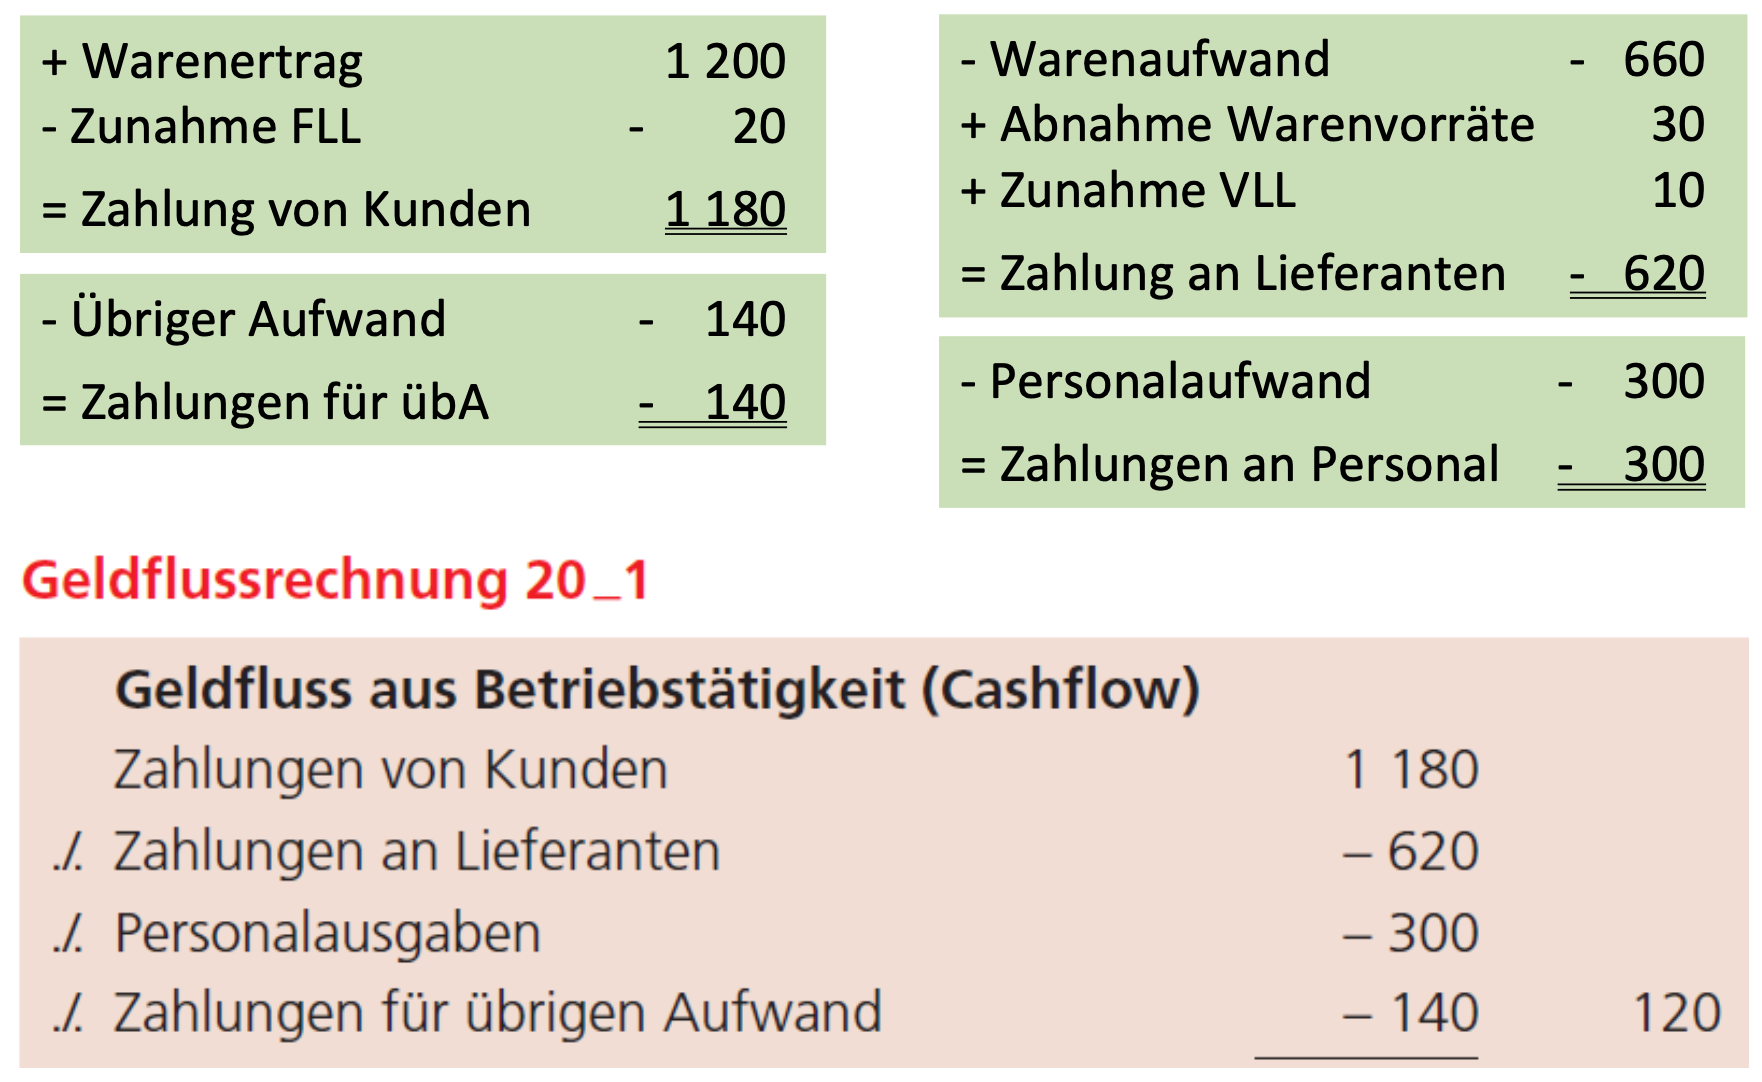
\includegraphics[width=\linewidth]{imgages/geldflussrechnung_direkt.png}\par}

\K{Indirekte Berechnung} (Ausgang Reingewinn): Reingewinn $+$ liq.-unwirksame Aufwände (z.B.\ Abschreibung) $-$ liq.-unwirksame Erträge $\pm$ Veränderung NUV (Umlaufvermögen \& kurzfr.\ FK).\\

{\centering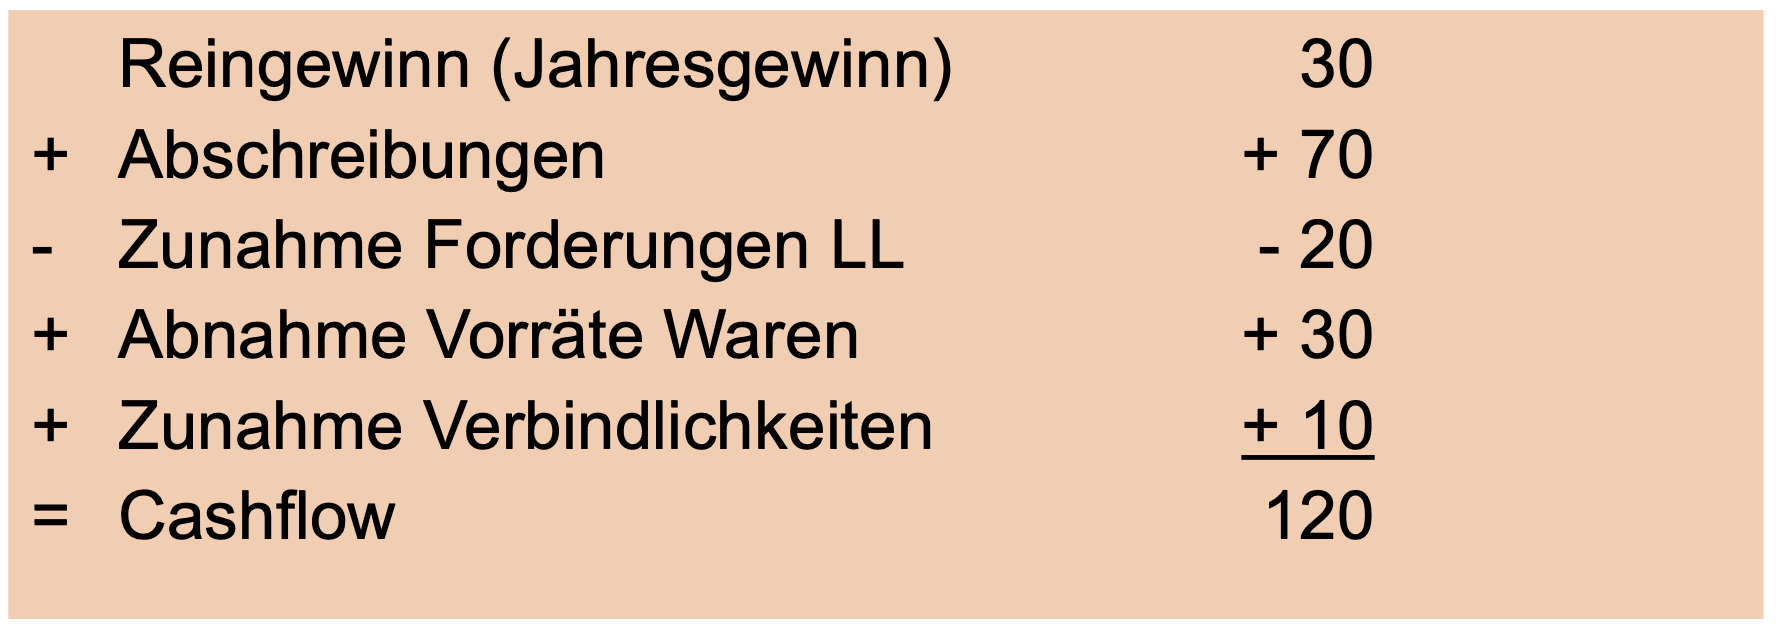
\includegraphics[width=\linewidth]{imgages/geldflussrechnung_indirekt.png}\par}

\K{Gesamte Geldflussrechnung}\\
{\centering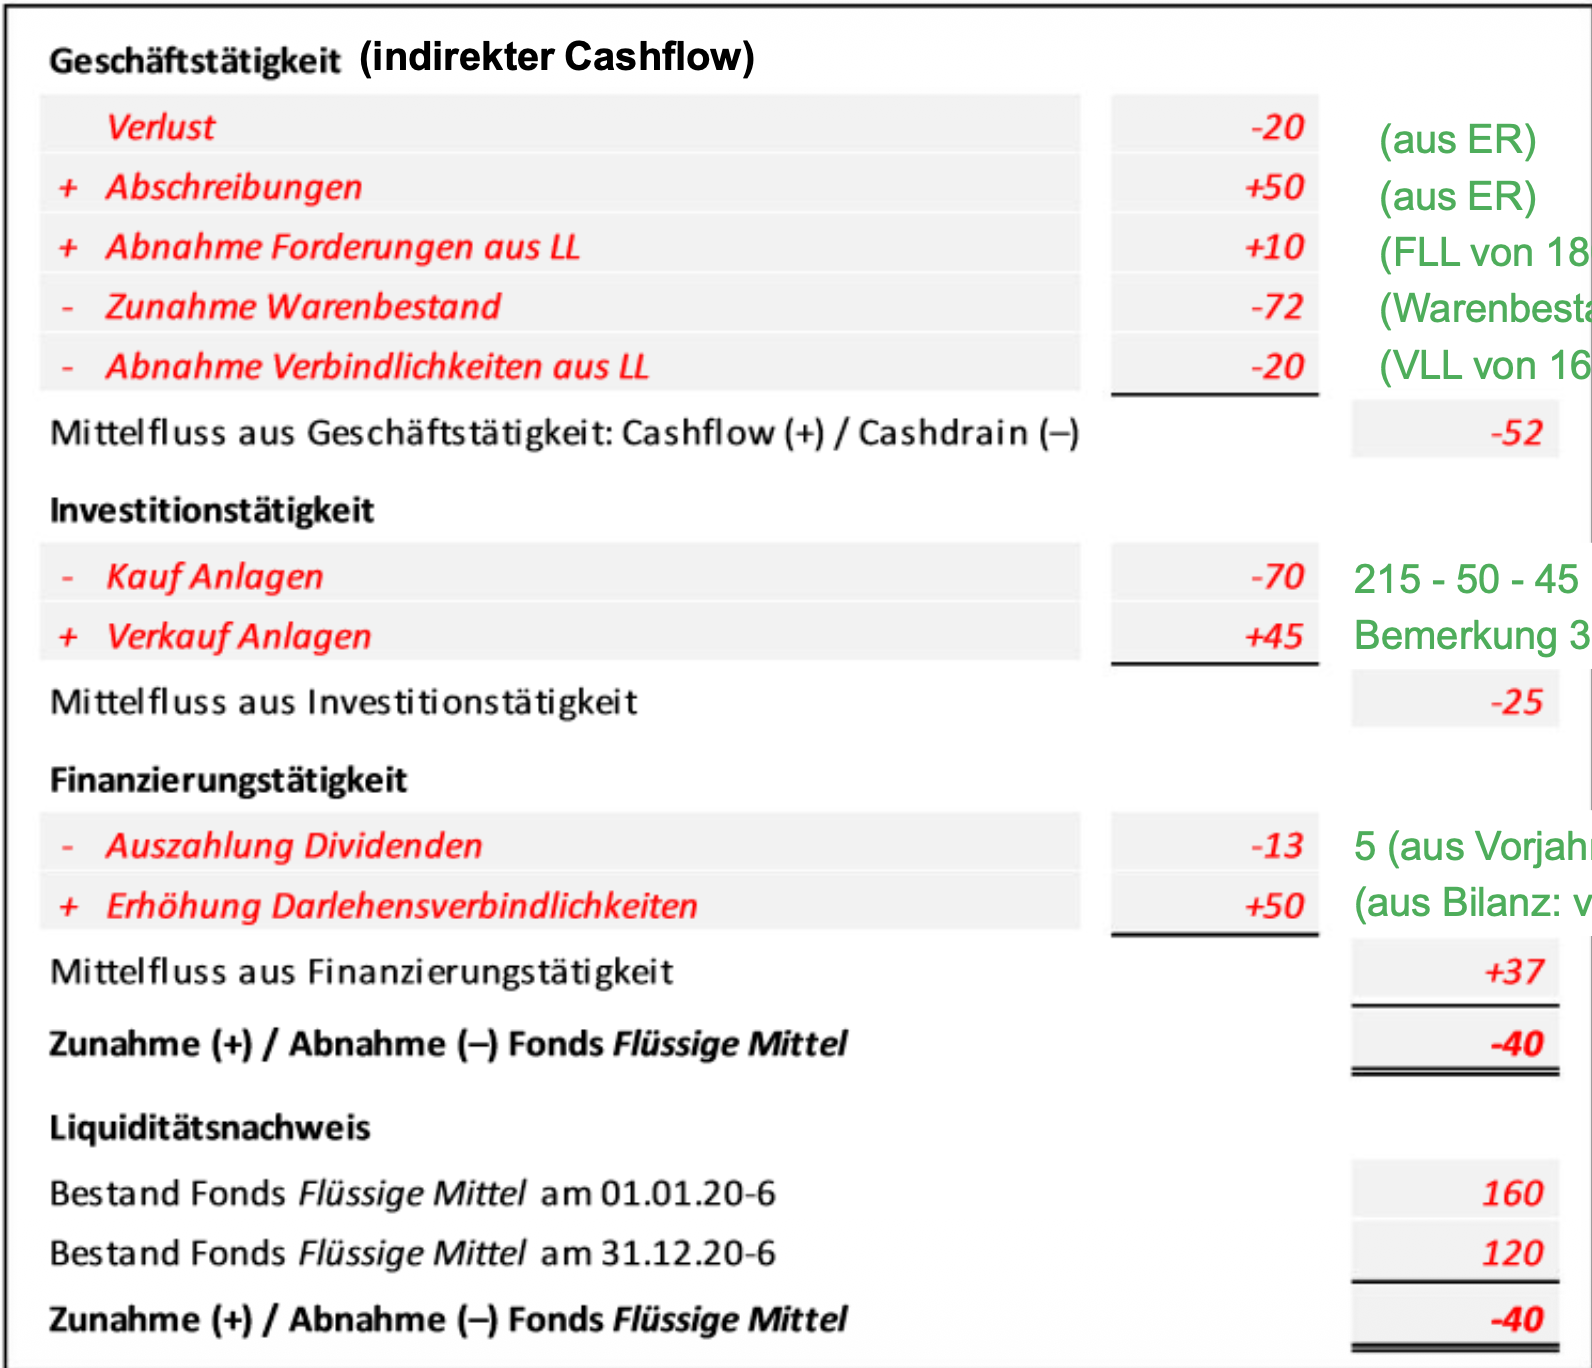
\includegraphics[width=\linewidth]{imgages/geldflussrechnung_gesamt.png}\par}
{\centering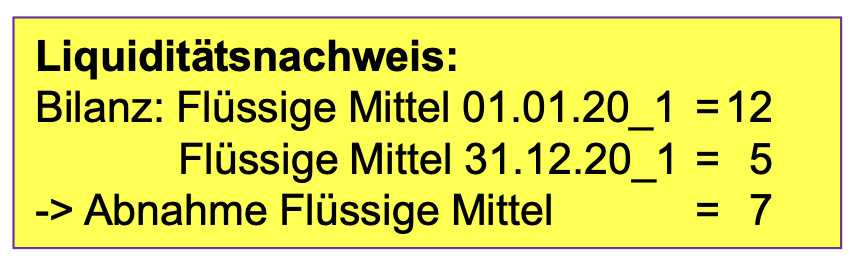
\includegraphics[width=0.7\linewidth]{imgages/liquiditaetsnachweis.png}\par}

\sechead{Finanzierung — Grundlagen}
{\centering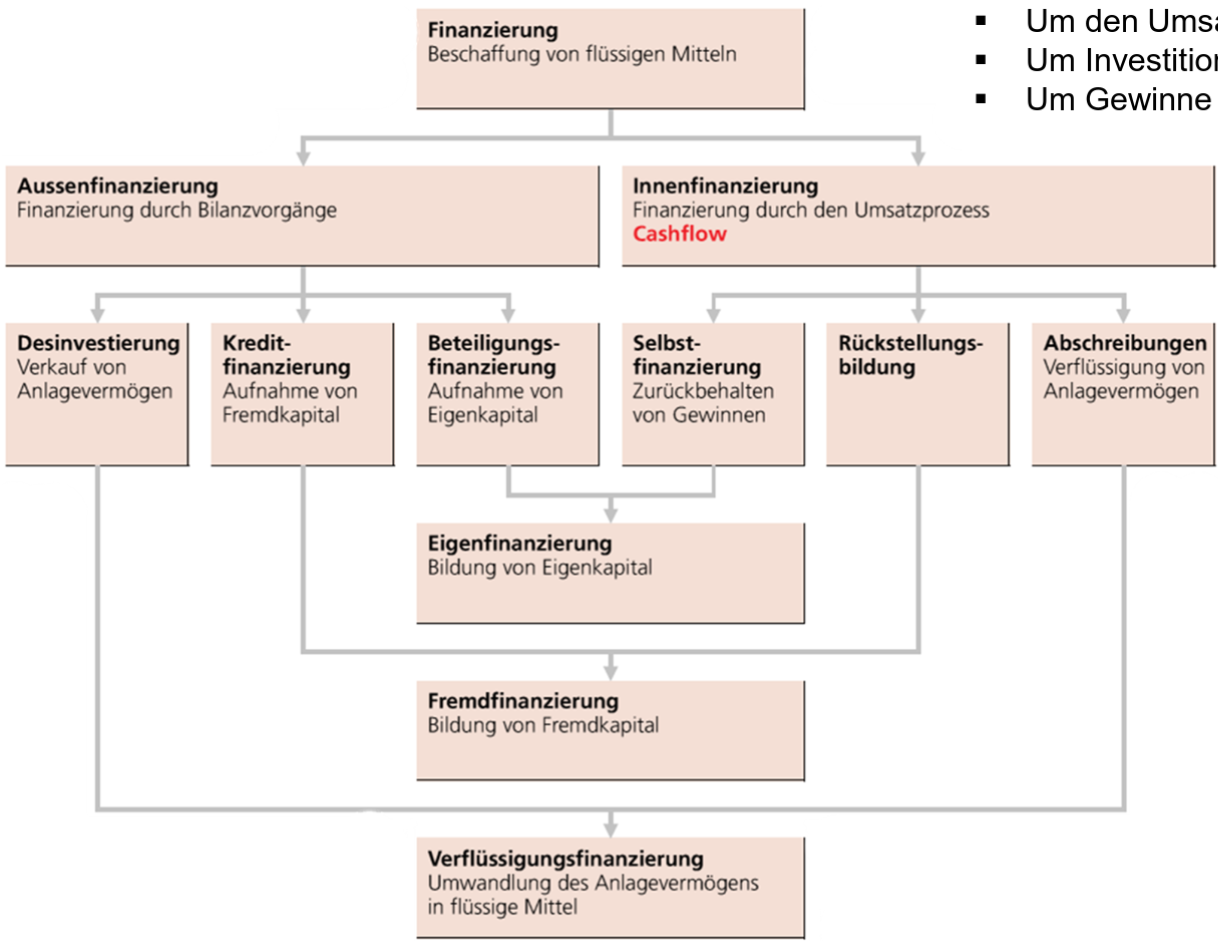
\includegraphics[width=\linewidth]{imgages/finanzierung.png}\par}

\K{Investition} = Mittel \emph{verwenden}.
Magisches Dreieck: Rendite–Sicherheit–Liquidität (+ Wachstum = Viereck).\\
\K{Bilanzwirkung}: Kapitalzuführung (Aussenfin., erhöht Bilanzsumme)
vs.\ Vermögensverflüssigung (Umschichtung, Bilanzsumme bleibt gleich).\\
\K{Crowdfunding}: -supporting (Spende), -investing (EK), -lending (FK).\\
\K{Going Public}: private AG $\to$ börsenkotiert (Kapitalbedarf decken, Risiko teilen).

\sechead{Finanzierungsformen}
\K{Kreditfinanzierung (FK)}: Anspruch auf Zins $+$ Rückzahlung.
\begin{itemize}
\item $+$ Elastizität, Zins senkt Steuer (Tax Shield), positiver \K{Leverage}
(EK-Rendite steigt mit FK, solange FK-Zins $<$ GK-Rendite).
\item $-$ Sicherheit/Bonität sinkt, künftiges FK teurer.
\item \emph{Kurzfr.}: Lieferanten-, Kunden-, Bankkredit, Factoring.
\emph{Langfr.}: Darlehen, Kassenobl., Hypothek, Wandelanleihe (Mezz.), Leasing (Finance-/Operating).
\end{itemize}
\K{Innenfinanzierung} (Ergänzung zur Grafik):
\begin{itemize}
\item \emph{Selbstfin.}: offen (Reserven) vs.\ verdeckt (stille Reserven).
\item \emph{Abschreibungsfin.}: Lohmann-Ruchti / Kapazitätserweiterungseffekt.
\item \emph{Rückstellungsfin.}: spätere Auszahlung, Steueraufschub.
\end{itemize}
\K{Beteiligungsfin.} (AK-Erhöhung): $+$ kein Fixzins, sehr langfr.\ Kapital, bessere Bonität;
$-$ Rentabilität sinkt, Dividende nicht steuerabzugsfähig.
Formen: Nennwert$\uparrow$, ordentl./bedingte Erhöhung, Kapitalband.\\
\K{Dividendenpolitik}: Bar-, Stock-, Naturaldividende;
stabil vs.\ gewinnabhängig.

\sechead{Kapitalkosten \& WACC}
\K{Fremdkapitalkosten} (über Bonität/Rating):\\
\fb{k_{FK}=r_f+\text{Credit Spread}}\\
$r_f$ = risikoloser Zins (10-J Bundesanleihe).
Besseres Rating $\Rightarrow$ tieferer Spread;
längere Laufzeit $\Rightarrow$ höherer Spread (Basispunkte).
Bei kotierten Firmen aus Anleihe-Coupons ablesbar.\\
\K{Eigenkapitalkosten (CAPM)} = verlangte Mindestrendite (RRR);
kalkulatorische Opportunitätskosten:\\
\fb{k_{EK}=r_f+\beta\,(r_M-r_f)}\\
$r_M$ = erw.\ Marktrendite ($\approx$8\%, SPI/Index);
$(r_M{-}r_f)$ = Marktrisikoprämie;
$\beta$ = systematisches Risiko (meist 0.5–2;
$\beta{=}1$ wie Markt, $\beta{>}1$ riskanter/zyklisch, $\beta{<}1$ defensiv z.B.\ Food/Pharma).
\K{Levered $\beta$} (inkl.\ Verschuldung) für CAPM;
\emph{unlevered} für Peer-Benchmarking.\\
\K{WACC} = $\varnothing$ gewichtete Kapitalkosten = Diskontsatz DCF = geforderte Mindestrendite:\\
\fb{\text{WACC}=k_{EK}\tfrac{EK}{GK}+k_{FK}\tfrac{FK}{GK}}\\
\fb{\text{WACC}_{tax}=k_{EK}\tfrac{EK}{GK}+k_{FK}\tfrac{FK}{GK}(1{-}t)}\\
$t$ = Steuersatz.
\K{Tax-Shield}: FK-Zins steuerlich abzugsfähig $\Rightarrow$ WACC$_{tax}$ tiefer.
$k_{EK}>k_{FK}$ (EK ist teurer).
WACC liegt zwischen $k_{FK}$ \& $k_{EK}$;
höherer Verschuldungsgrad $\Rightarrow$ höhere FK-Kosten.
\begin{exbox}
$k_{EK}{=}16\%,k_{FK}{=}9\%,EK{=}60\% \\
FK{=}40\%,t{=}40\%$:\\
WACC $=16{\cdot}0.6+9{\cdot}0.4=\R{13.2\%}$\\
WACC$_{tax}=9.6+9{\cdot}0.4{\cdot}0.6=\R{11.76\%}$\\[2pt]
\textbf{CAPM$\to$WACC}: $r_f{=}2\%,\beta{=}0.8,r_M{=}7\%$, \\
EK 14, FK 6, $t{=}20\%$:\\
$k_{EK}=2+0.8{\cdot}5=6\%$\\
WACC$_{tax}=6{\cdot}0.7+5{\cdot}0.3{\cdot}0.8=\R{5.4\%}$
\end{exbox}

\sechead{Investitionsrechnung}
Investition = Verwendung liquider Mittel für dauerhafte Gegenstände (AV);
sichere Auszahlung heute $\to$ unsichere Rückflüsse später ($\Rightarrow$ Risiko).\\
\K{Arten}: Sach-, immaterielle, Finanzanlage-Investition.\\
\K{Anlässe}: Gründung, Ersatz, Erweiterung, Rationalisierung.\\
\K{Methoden}: \emph{statisch} (ohne Zeitwert)
vs.\ \emph{dynamisch} (mit Zeitwert/Diskontierung).
Dynamisch theoretisch überlegen;
statisch in der Praxis als Überschlag dennoch verbreitet.\\


% \K{Projektspezifischer WACC (Hurdle Rate)}: $\beta$ je Projekt/Technologie (via Peer Group bzw.\ Expertenpanel) anpassen;
% FK-Kosten konzernabhängig.
% \K{Szenarien} (Best-guess / Worst / Optimistic) für zentrale Treiber (Nachfrage, Preise, Marge)
% $\Rightarrow$ Sensitivität testen.
% Nominaler WACC $\Rightarrow$ alle Cashflows inflationieren.

\sechead{Statische Methoden}
\emph{Zeitwert des Geldes wird NICHT berücksichtigt.}\\
\K{Kostenvergleich} (niedrigste $\varnothing$-Kosten/Jahr gewinnt):\\
\fb{\text{kalk.\ Abschr.}=\tfrac{AnschKosten-RestWert}{Nutzungsdauer}}\\
\fb{\varnothing\text{geb.\ Kapital}=\tfrac{AnschKosten+RestWert}{2}}\\
\fb{\text{kalk.\ Zinsen}=\varnothing\text{geb.\ Kapital}\cdot i}\\
Gesamtkosten $=$ Fixkosten (kalk.\ Abschr.\ $+$ Zinsen $+$ sonst.\ Fix) $+$ variable Kosten.
\emph{Sagt nichts über Erlöse aus.}\\
\K{Rentabilität (ROI)} (höchster gewinnt):\\
\fb{\text{ROI}=\dfrac{\text{Gewinn}+\text{kalk.\ Zinsen}}{\varnothing\text{-Kapital}}\cdot100}\\
Gewinn $=$ Erlöse $-$ Gesamtkosten.\\
\K{Statische Payback} (kürzeste Dauer;
lohnt, wenn $<$ ND/Schwellenwert):\\
\fb{\text{Payback}=\dfrac{K_0}{\varnothing\,\text{Cashflow}}}\\
CF $=$ Gewinn $+$ Abschr.\ $+$ Zins.
\emph{Durchschnitts-} (gleicher CF) / \emph{Kumulationsmethode} (jährl.\ CF abziehen bis $K_0$ gedeckt).
Misst Risiko \& Liquidität, nicht Gesamtrendite.
\begin{exbox}
\textbf{Kostenvergleich LKW} (AK 23'000, RW 10\%$=$2'300, ND 8 J, $i$ 5\%):\\
kalk.\ Abschr.\ $=\tfrac{23'000-2'300}{8}=2'588$\\
$\varnothing K=\tfrac{23'000+2'300}{2}=12'650$\\
kalk.\ Zins $=12'650{\cdot}0.05=633$\\
$\Rightarrow$ in Fixkosten einrechnen, dann $+$ variable Kosten vergleichen.
\end{exbox}
\begin{exbox}
\textbf{Payback}: $K_0$ 7.5 Mio, CF (1.0$+$0.4$+$0.1)$=$1.5 $\Rightarrow$ $7.5/1.5=\R{5\,\text{J}}$\\[2pt]
\textbf{ROI Masch.}: $\varnothing K$ 40'000, Gewinn 17'000, Zins 2'400:\\
$\tfrac{17'000+2'400}{40'000}{\cdot}100=\R{48.5\%}$
\end{exbox}

\sechead{Dynamische Methoden}
\emph{Zeitwert: 1 CHF heute $>$ 1 CHF morgen.} Gerechnet wird mit \K{Cashflows} (operativ, \emph{ohne} Zinskosten);
Liquidationserlös $=$ CF des letzten Jahres.\\
\K{Barwert (PV)}:\\
\fb{PV=\dfrac{CF_n}{(1+R)^n}=CF_n\cdot\text{AbF}}\\
\K{Annuität/Rente} (konstanter CF): \fb{PV=CF\cdot\text{RBF}_{R,T}}\\
$R$ = Diskontsatz = WACC.
RBF $=\sum$AbF (ab J1);
ewig RBF$_\infty=\tfrac1R$.\\
\K{Kapitalwert (NPV / NBW)}:\\
\fb{\text{NPV}=-K_0+\sum_{n=1}^{T}\dfrac{CF_n}{(1+R)^n}}\\
\R{NPV $>$ 0 $\Rightarrow$ lohnt sich} (steigert Unternehmenswert);
NPV $<$ 0 $\Rightarrow$ nein.
$K_0$ wird \emph{nicht} diskontiert (J0).\\
\K{NPV-Koeffizient} (bei untersch.\ $K_0$): \fb{\tfrac{\text{NPV}}{K_0}} (höchster gewinnt).\\
\K{Operativen CF aufbauen} (häufige Rechenaufgabe):\\
Menge $\times$ Preis $=$ Umsatz;
$-$ variable Kosten (Material, etc.\ je Stk) $-$ Fixkosten $=$ Cashflow (\emph{ohne} Abschr.\ \& Zins).
Einmalige Posten (z.B.\ Grossrevision) im jeweiligen Jahr abziehen, Liquidationserlös im letzten Jahr addieren.
\begin{exbox}
\textbf{CF-Aufbau}: 300'000 Stk $\times$ 28 $=$ 8.4 Mio Umsatz;
var.\ (8$+$5)$\times$300'000 $=$ 3.9 Mio;
Fix 4.0 Mio
$\Rightarrow$ CF $=8.4-3.9-4.0=\R{0.5\,\text{Mio/J}}$.
Dann je Jahr diskontieren $\to$ NPV.
\end{exbox}
\begin{exbox}
\textbf{Taxi}: $K_0$ 42'000;
CF 9'000 (J1–5), Restwert 17'000 in J5;
$R{=}8\%$;
RBF$_5{=}3.993$, AbF$_5{=}0.681$.\\
PV $=9'000{\cdot}3.993+17'000{\cdot}0.681$\\
$=35'937+11'577=47'514$\\
NPV $=47'514-42'000=\R{+5'514}$
\end{exbox}
\begin{exbox}
\textbf{Anlage V} (175'000/J, 10 J, $K_0$ 937'000, 8\%, RBF$_{10}{=}6.710$):\\
$175'000{\cdot}6.710=1'174'250$;\\
NPV $=1'174'250-937'000=\R{+237'250}$
\end{exbox}
\K{Interner Zinssatz (IRR)}: Zins, bei dem NPV $=0$:\\
\fb{0=-K_0+\sum_{n=1}^{T}\dfrac{CF_n}{(1+IRR)^n}}\\
Bei Annuität: $\text{RBF}=\tfrac{K_0}{CF}$, zu $T$ den Zins in RBF-Tabelle suchen \& \K{linear interpolieren}:\\
\fb{IRR=i_1+\dfrac{\text{RBF}_{i_1}-\text{RBF}}{\text{RBF}_{i_1}-\text{RBF}_{i_2}}(i_2{-}i_1)}\\
\R{IRR $\geq$ WACC $\Rightarrow$ vorteilhaft.} Anschaulicher als NPV;
Vorsicht beim Projektvergleich: NPV \& IRR können unterschiedlich rangieren (untersch.\ Wiederanlage-Annahme) — \R{NPV entscheidet}.
\begin{exbox}
$K_0$ 13'000, CF 5'000, $T{=}3$: RBF $=2.6$.\\
3 J: 7\%$\to$2.624, 8\%$\to$2.577.\\
IRR $=7+\tfrac{2.624-2.6}{2.624-2.577}=\R{7.51\%}$\\
$<$ 8\% gefordert $\Rightarrow$ \emph{nicht} rentabel.
\end{exbox}
\K{Annuitätenmethode}: konstanter CF, der bei gegeb.\ $K_0$ genau $R$ erwirtschaftet (NPV$=0$);
$\text{Annuität}=K_0/\text{RBF}$ (z.B.\ Leasingrate).\\
\K{Dynamische Payback}: diskontierte CF kumulieren bis $K_0$ gedeckt (länger als statisch).\\
\K{Net Present Costs (NPC)}: Barwert aller Kosten $+K_0$ (Systemvergleich, z.B.\ Heizung;
Restwert im letzten Jahr abziehen).
NPV $=$ Barwert aller \emph{Cashflows} (Einnahmen $-$ Kosten).

\sechead{Unternehmensbewertung}
\K{Wert $\neq$ Preis} (Preis durch Verhandlung/Markt;
``mehr Kunst als Wissenschaft'', Bandbreite).
Anlässe: M\&A, IPO, Start-up-Finanzierung, Nachfolge.\\
\K{Entity} = Brutto-UW (EK$+$FK), Diskont WACC;
\K{Equity} = Netto-UW (nur EK), Diskont $k_{EK}$.\\[2pt]
\K{Substanzwert} (gegenwartsorientiert, oft Wertuntergrenze):\\
\fb{\text{Brutto-SW}=\text{Aktiven}+\text{stille Res.}}\\
\fb{\text{Netto-SW}=\text{Brutto-SW}-FK}\\
Stille Reserven = Unterbewertung Aktiven oder Überbewertung Passiven.
$+$ anlageintensive Branchen/Banken;
$-$ vernachlässigt Zukunft \& Risiko, untauglich für wachstumsstarke Firmen.
\begin{exbox}
\textbf{Substanzwert} (Mio): Vorräte Bilanz 300/Markt 320 ($+$20), AV 1'200/1'400 ($+$200), übrige 200/200;
FK 950.\\
Brutto-SW $=1'700+220=1'920$\\
Netto-SW $=1'920-950=\R{970}$\\
$=$ EK 750 $+$ stille Res.\ 220
\end{exbox}
\K{Ertragswert} (ewige Rente, Nullwachstum, Equity):\\
\fb{UW_0=\dfrac{\text{nachh.\ ber.\ RG}}{k_{EK}}}\\
RG bereinigen um ao./einmalige Posten (z.B.\ Auflösung Rückstellung), Steuern neu rechnen, $\varnothing$ letzte 3–5 Jahre.
KMU-Diskont pragmatisch: $r_f$ $+$ Marktprämie $+$ Zuschläge (klein/illiquide/spezifisch)
$\Rightarrow$ 7–25\%.
Start-ups 15–70\%.
\begin{exbox}
\textbf{Kägifrett}: nachh.\ Gewinn 1.65 Mio, EK-Rendite 11\%:\\
EW $=1.65/0.11=\R{15\,\text{Mio.}}$\\
\footnotesize (reiner Ertragswert: $k_{EK}$, nicht WACC!)
\end{exbox}
\begin{exbox}
\textbf{Bereinigter RG} (Mio): RG 95, Steuer 41 ($t$ 30\%), Auflösung Rückstellung 6 (einmalig).\\
EBT $=95+41=136$;
$-$ 6 (ao.) $=$ 130 nachh.\ Vorsteuergewinn;
$-$ 30\% Steuer $(39)$ $=\R{91}$ bereinigter RG.
\end{exbox}
\K{Mittelwert (Praktiker)}: Substanz \& Ertrag, EW in CH oft doppelt:\\
\fb{UW_0=\dfrac{2\cdot EW+1\cdot\text{Netto-SW}}{3}}
\begin{exbox}
\textbf{Spyder}: Bilanzsumme 410, stille Res.\ $15{+}10{+}10{+}40{=}75$, FK 335;
$\varnothing$RG $(42{+}35{+}31)/3{=}36$;
$k_{EK}{=}12\%$.\\
Brutto-SW $=410+75=485$\\
Netto-SW $=485-335=150$\\
EW $=36/0.12=300$\\
MW $=(2{\cdot}300+150)/3=\R{250\,\text{Mio.}}$
\end{exbox}
\K{DCF-Methode} (Best Practice, Entity, Free Cashflow).
FCF aus EBIT (nicht Reingewinn!):\\
\fb{\text{NOPAT}=EBIT\,(1{-}t)}\\
\begin{tabular}{@{}r@{~}l@{}}
 & NOPAT\\
$+$ & Abschreibungen / nicht-lw\\
$\mp$ & Veränderung NUV (betriebl.)\\
$-$ & Investitionen $+$ Desinvest.\\
$=$ & \K{Free Cashflow (FCF)}\\
\end{tabular}\\
NUV $=$ UV $-$ kurzfr.\ FK (nur betriebl.\ Positionen, ohne flüssige Mittel).
FCF \emph{vor} Zinsen (steht auch FK-Gebern zur Verfügung).
\begin{exbox}
\textbf{FCF-Aufbau} (EBIT 1'000, $t$ 20\%): NOPAT $=1'000{\cdot}0.8=800$;
$+$ Abschr.\ 200 $=$ 1'000;
$-$ Zunahme NUV 100 $=$ 900;
$-$ Investition 300 $=$ \R{FCF 600}.
\end{exbox}
\fb{\text{Brutto-UW}=\sum_{n=1}^{T}\dfrac{FCF_n}{(1{+}w)^n}+\dfrac{TV}{(1{+}w)^T}}\\
($w=$ WACC$_{tax}$)\\
\K{Terminal Value} — Nullwachstum: \fb{TV=\dfrac{FCF}{w}};
mit Wachstum $g$: \fb{TV=\dfrac{FCF\,(1+g)}{w-g}}\\
\fb{\text{Equity}=\text{Brutto-UW}-FK}\\
TV als Cashflow zum Zeitpunkt $T$ mitdiskontieren.
3-Phasen: Detail-, Übergangs-, Endphase.
``Profit is opinion, cash is fact.'' $-$ hohes Gewicht des TV, Prognoseunsicherheit.
\begin{exbox}
\textbf{TV-Vergleich} (FCF$_T$ 1'400, $w{=}10\%$):\\
Nullwachstum $=1'400/0.10=\R{14'000}$\\
$g{=}3\%$: $\tfrac{1'400\cdot1.03}{0.10-0.03}=\R{20'600}$
\end{exbox}
\K{Multiplikator (relativ)}: Netto-UW $=$ Kennzahl $\times$ Multiple (aus Peers/Branche).
\begin{itemize}
\item Umsatz ($0.5$–$1.2$): auch bei Verlustfirmen/Start-ups.
\item EBITDA ($4$–$9$): wenn keine grossen Investitionen nötig.
\item EBIT ($5$–$10$): glättet Investitionen via Abschr.
\end{itemize}
Kotiert: \fb{\text{KGV}=\tfrac{\text{Kurs}}{\text{Gewinn/Aktie}}}, \fb{\text{KBV}=\tfrac{\text{Kurs}}{\text{Buchwert/Aktie}}}.
EV/EBITDA in CH am beliebtesten.
Hohes KGV $\Rightarrow$ stark erwartetes Wachstum.
\begin{exbox}
\textbf{Multiple}: EBITDA 0.5 Mio, EBITDA-Multiple 6
$\Rightarrow$ Netto-UW $=0.5{\cdot}6=\R{3\,\text{Mio.}}$\\
KGV-Bsp.: Kurs 80, Gewinn/Aktie 4
$\Rightarrow$ KGV $=20$.
\end{exbox}
\K{Goodwill} $=$ Transaktionspreis $-$ Netto-Substanzwert (Mehrwert: Know-how, Marke, Kunden, Management).
Derivativer GW wird aktiviert, originärer (selbst erarbeitet) nicht.
\begin{exbox}
\textbf{Goodwill}: Preis 12 Mio, Netto-SW 9.5 Mio
$\Rightarrow$ GW $=12-9.5=\R{2.5\,\text{Mio.}}$
\end{exbox}

\sechead{Ergänzungen \& Würdigung}
\K{Invest.-rechnung vs.\ Bewertung}: gleiches Prinzip (Diskontieren künftiger Zahlungen), aber Investition $=$ einzelnes Projekt (begrenzte ND), Bewertung $=$ ganzes Unternehmen (oft ewig, Terminal Value).\\
\K{NPV vs.\ IRR (Konflikt)}: bei sich ausschliessenden Projekten können NPV \& IRR unterschiedlich rangieren (untersch.\ Wiederanlage-Annahme).
\R{NPV entscheidet} (misst absoluten Wertbeitrag);
IRR bevorzugt Projekte mit frühen/hohen CF.\\
\K{Würdigung}: Substanzwert bestandesorientiert (Untergrenze);
Ertragswert konservativ (Nullwachstum, manipulierbarer Gewinn);
DCF Best Practice, aber TV-lastig \& prognoseabhängig;
Multiplikator schnell, aber Peer-abhängig.\\
\K{NPC-Bsp.}: Investition 16'000 (J0) $+$ jährl.\ Kosten 2'867 über ND, mit $R$ diskontiert, $-$ Restwert im letzten Jahr
$\Rightarrow$ tiefste NPC gewinnt (z.B.\ Wärmepumpe vs.\ Gas).

\begin{tcolorbox}[colback=cBox,colframe=cA,boxrule=0.35pt,left=2.5pt,right=2.5pt,top=2pt,bottom=2pt,arc=1pt]
\textbf{Begriffe (Glossar)}\\
\K{EBITDA}: Betriebsergebnis vor Zinsen, Steuern, Abschr.\\
\K{EBIT}: Betriebsgewinn (nach Abschr., vor Zins/Steuer).\\
\K{EBT}: Gewinn vor Steuern.\\
\K{NOPAT}: $EBIT(1{-}t)$, Betriebsgewinn nach approx.\ Steuern, vor Zins.\\
\K{FCF}: Free Cashflow, steht EK $+$ FK-Gebern zur Verfügung (Entity).\\
\K{NUV}: Nettoumlaufverm.\ $=$ UV $-$ kurzfr.\ FK (betriebl.).\\
\K{Tax Shield}: Steuerersparnis durch abzugsfähige FK-Zinsen.\\
\K{Leverage}: EK-Rendite$\uparrow$ durch FK, solange FK-Zins $<$ GK-Rendite.\\
\K{WACC}: gewichtete $\varnothing$-Kapitalkosten $=$ geforderte Mindestrendite.\\
\K{Credit Spread}: Risikozuschlag (Rating) auf $r_f$.\\
\K{$\beta$}: systematisches (Markt-)Risiko einer Aktie.\\
\K{Goodwill}: Preis $-$ Netto-Substanzwert (immat.\ Mehrwert).\\
\K{Stille Reserven}: Unterbew.\ Aktiven / Überbew.\ Passiven.\\
\K{Substanz-/Ertrags-/DCF-Wert}: Vergangenheit / konstanter Gewinn / künftige Free Cashflows.
\end{tcolorbox}

% ============ EXAM-TRAPS ============
\begin{tcolorbox}[colback=cWarn,colframe=red!55!black,boxrule=0.35pt,left=2.5pt,right=2.5pt,top=2pt,bottom=2pt,arc=1pt]
\textbf{MC-Fallen (Kprim, richtig/falsch)}\\
\R{F:} ``Statische Methoden berücksichtigen Zeitpunkte künftiger Werteflüsse'' — nur \emph{dynamische}.\\
\R{R:} Software-Update-Kosten senken Gewinn \emph{und} Cashflow (liq.-wirksamer Aufwand).\\
\R{R:} Direkte Cashflow-Berechnung berücksichtigt kalkulatorische Zinsen nicht.\\
\R{R:} Kapitaleinsatz $>$ Summe abgezinster CF
$\Rightarrow$ NPV$<$0
$\Rightarrow$ lohnt nicht.\\
\R{F:} ``WACC = erwartete/erzielte Rendite'' — WACC ist \emph{geforderte} Mindestrendite/Kosten.\\
\R{F:} ``WACC nur bei Equity-Ansätzen'' — WACC gehört zum Entity-/DCF-Ansatz;
Equity nutzt $k_{EK}$.\\
\R{R:} WACC = Mindestrendite, damit es sich für die Kapitalgeber lohnt.\\
\R{R:} WACC = gewichtete $\varnothing$-Kosten von Eigen- \& Fremdkapital.\\
\R{R:} EK ist teurer als FK ($k_{EK}>k_{FK}$);
höherer Verschuldungsgrad erhöht FK-Kosten.
\end{tcolorbox}

% ============ FAKTOR-MERKHILFE ============
\begin{tcolorbox}[colback=cBox,colframe=cA,boxrule=0.35pt,left=2.5pt,right=2.5pt,top=2pt,bottom=2pt,arc=1pt]
\textbf{Faktor-Logik} (Tabellen separat mitnehmen!)\\
AbF$_{R,n}=\dfrac{1}{(1+R)^n}$ — einzelnes Jahr abzinsen.\\
RBF$_{R,T}=\sum_{n=1}^{T}$AbF — konstante Rente;
RBF$_\infty=\tfrac1R$.\\
RBF mit Wachstum: $\tfrac{1}{R-g}$ (ewig).\\[3pt]
\textbf{Rechenaufgaben:} Schritte einzeln \& nachvollziehbar notieren (nur $+\ -\ /\ \hat{}\ ()$ ), Zwischenwerte runden wie verlangt, Endergebnis klar markieren.
\R{Teilpunkte trotz falschem Endergebnis!} Einheiten \& Vorzeichen prüfen.
\end{tcolorbox}

\begin{tcolorbox}[colback=cEx,colframe=cB!70!black,boxrule=0.35pt,left=2.5pt,right=2.5pt,top=2pt,bottom=2pt,arc=1pt]
\textbf{Welche Methode wann?}\\
\R{Investition lohnt sich?}
$\to$ NPV/IRR (dyn.), Payback, ROI.\\
\R{Projektwahl, gleiches $K_0$}
$\to$ höchster NPV.\\
\R{Projektwahl, untersch.\ $K_0$}
$\to$ NPV-Koeffizient.\\
\R{Anlageintensiv / Untergrenze}
$\to$ Substanzwert.\\
\R{Stabile Gewinne, KMU}
$\to$ Ertragswert / Mittelwert.\\
\R{Wachstum, Konzern, M\&A}
$\to$ DCF (Best Practice).\\
\R{Schneller Marktvergleich}
$\to$ Multiplikator.\\
\R{Systemkosten-Vergleich}
$\to$ NPC.\\[3pt]
\textbf{Diskontsatz:} Investition/DCF/Brutto-UW
$\to$ \K{WACC};
reiner Ertragswert/Equity
$\to$ \K{$k_{EK}$}.
\end{tcolorbox}

\begin{tcolorbox}[colback=cBox,colframe=cA,boxrule=0.35pt,left=2.5pt,right=2.5pt,top=2pt,bottom=2pt,arc=1pt]
\textbf{Weitere Begriffe (MC-relevant)}\\
\K{Geldmarkt} ($<$1\,J: Fest-/Termingeld)
vs.\ \K{Kapitalmarkt} ($>$1\,J: Obligationen, Aktien, Hypotheken).\\
\K{Weitere Multiples}: EBITC (Gewinn $+$ GF-Lohn), KCV (Kurs/Cashflow), KUV (Umsatz), KDV (Dividende);
\K{EV} $=$ Enterprise Value $=$ Brutto-UW.\\
\K{Skonto} bei Lieferantenkrediten nutzen (Innenfin.\ des UV).\\
\K{Basel III}: Banken müssen EK erhöhen.\\
\K{Impairment-Test} (IFRS): jährl.\ Buchwert vs.\ Marktwert
$\to$ ggf.\ Abschreibung.\\
\K{AK-Erhöhung}: ordentlich (GV, VR 3 Mt.), bedingt (Wandel-/Optionsrechte), Kapitalband (VR, 5 J).\\
\K{Real vs.\ nominal WACC}: real $=$ inflationsbereinigt;
bei nominalem WACC alle Cashflows inflationieren.\\
\K{$\beta$ levered} (inkl.\ Verschuldung, für CAPM)
vs.\ \K{unlevered} (für Peer-Benchmark, dann relevern).
\end{tcolorbox}

\end{multicols}

% =================== SEITE 4: REINE FORMELSAMMLUNG ===================
\clearpage
\begin{multicols}{4}
\normalsize
\setlength{\parskip}{2.5pt}
{\centering\colorbox{cA}{\color{white}\bfseries\,FORMELSAMMLUNG — Investition \& Finanzierung\,}\par}
\vspace{2pt}

\K{Bilanz / Erfolgsrechnung}\\
\fb{\text{Aktiven}=\text{Passiven}}\quad\fb{EK=\text{Aktiven}-FK}\\
EBITDA $\xrightarrow{-\text{Abschr.}}$ EBIT $\xrightarrow{-\text{Zins}}$ EBT $\xrightarrow{-\text{Steuer}}$ RG\\
\fb{\text{Verschuldungsgrad}=\tfrac{FK}{GK}}\quad\fb{\text{EK-Quote}=\tfrac{EK}{GK}}

\K{Cashflow (indirekt)}\\
\fb{CF=RG+\text{Abschr.}\pm\text{nicht-lw}\mp\Delta\text{Akt.}\pm\Delta\text{Pass.}}\\
AV: \fb{AB-\text{Abschr.}+\text{Inv.}-\text{Desinv.}=SB}

\K{Kapitalkosten}\\
\fb{k_{FK}=r_f+\text{Credit Spread}}\\
\fb{k_{EK}=r_f+\beta\,(r_M-r_f)}\\
\fb{\text{WACC}=k_{EK}\tfrac{EK}{GK}+k_{FK}\tfrac{FK}{GK}}\\
\fb{\text{WACC}_{tax}=k_{EK}\tfrac{EK}{GK}+k_{FK}\tfrac{FK}{GK}(1{-}t)}

\K{Statisch}\\
\fb{\text{kalk.\ Abschr.}=\tfrac{AK-RW}{ND}}\\
\fb{\varnothing K=\tfrac{AK+RW}{2}}\quad\fb{\text{Zins}=\varnothing K\cdot i}\\
\fb{\text{ROI}=\tfrac{\text{Gewinn}+\text{kalk.\ Zins}}{\varnothing K}\cdot100}\\
\fb{\text{Payback}=\tfrac{K_0}{\varnothing\,CF}}

\K{Dynamisch}\\
\fb{PV=\tfrac{CF_n}{(1+R)^n}=CF_n\cdot\text{AbF}}\\
\fb{PV=CF\cdot\text{RBF}_{R,T}}\quad\fb{\text{RBF}_\infty=\tfrac1R}\\
\fb{\text{NPV}=-K_0+\sum_{n=1}^{T}\tfrac{CF_n}{(1+R)^n}}\\
\fb{\text{NPV-Koeff}=\tfrac{\text{NPV}}{K_0}}\\
\fb{0=-K_0+\sum\tfrac{CF_n}{(1+IRR)^n}}\\
IRR (Annuität): \fb{\text{RBF}=\tfrac{K_0}{CF}}\\
\fb{IRR=i_1+\tfrac{\text{RBF}_{i_1}-\text{RBF}}{\text{RBF}_{i_1}-\text{RBF}_{i_2}}(i_2{-}i_1)}\\
\fb{\text{Annuität}=\tfrac{K_0}{\text{RBF}}}

\K{Bewertung}\\
\fb{\text{Brutto-SW}=\text{Aktiven}+\text{stille Res.}}\\
\fb{\text{Netto-SW}=\text{Brutto-SW}-FK}\\
\fb{\text{Ertragswert}=\tfrac{\text{nachh.\ ber.\ RG}}{k_{EK}}}\\
\fb{\text{Mittelwert}=\tfrac{2\,EW+1\,\text{Netto-SW}}{3}}\\
\fb{\text{NOPAT}=EBIT\,(1{-}t)}\\
FCF $=$ NOPAT $+$ Abschr.\ $\mp\Delta$NUV $-$ Inv.\ $+$ Desinv.\\
\fb{\text{Brutto-UW}=\sum\tfrac{FCF_n}{(1{+}w)^n}+\tfrac{TV}{(1{+}w)^T}}\\
\fb{TV=\tfrac{FCF}{w}}\quad\fb{TV=\tfrac{FCF(1+g)}{w-g}}\\
\fb{\text{Equity}=\text{Brutto-UW}-FK}\\
\fb{\text{Netto-UW}=\text{Kennzahl}\times\text{Multiple}}\\
\fb{\text{KGV}=\tfrac{\text{Kurs}}{\text{Gewinn/Aktie}}}\quad\fb{\text{KBV}=\tfrac{\text{Kurs}}{\text{Buchwert/Aktie}}}\\
\fb{\text{Goodwill}=\text{Preis}-\text{Netto-SW}}

\K{Vorzeichen \& Entscheid (Merker)}
\begin{itemize}
\item NPV $>0$ / IRR $\geq$ WACC $\Rightarrow$ Investition \R{lohnt sich}.  \item höchster NPV (gleiches $K_0$) bzw.\ höchster NPV-Koeffizient (untersch.\ $K_0$) gewinnt.  \item Cashflow-Aufbau (dyn.): Menge$\times$Preis $-$ var.\ Kosten $-$ Fixkosten ($+$Restwert im letzten Jahr), \emph{ohne} Abschr.\ \& Zins.  \item NUV $=$ UV $-$ kurzfr.\ FK (nur betriebl.).  \item kalk.\ Zinsen: nur statisch \& Kostenvergleich, nie im Cashflow.  \item Diskontsatz: DCF/Brutto-UW $\to$ WACC$_{tax}$; Ertragswert/Equity $\to k_{EK}$.  \end{itemize} \begin{tcolorbox}[colback=cBox,colframe=cA,boxrule=0.35pt,left=3pt,right=3pt,top=2.5pt,bottom=2.5pt,arc=1pt]
\textbf{Mini-Faktoren} (sonst Tabellen nutzen)\\[2pt]
\renewcommand{\arraystretch}{1.15}
\begin{tabular}{@{}l|cc|cc@{}}
 & \multicolumn{2}{c|}{AbF $\tfrac{1}{(1{+}R)^n}$} & \multicolumn{2}{c}{RBF $\sum$AbF}\\
$n$ & 5\% & 8\% & 5\% & 8\%\\\hline
1 & 0.952 & 0.926 & 0.952 & 0.926\\
3 & 0.864 & 0.794 & 2.723 & 2.577\\
5 & 0.784 & 0.681 & 4.329 & 3.993\\
10 & 0.614 & 0.463 & 7.722 & 6.710\\
$\infty$ & — & — & 20.0 & 12.5\\
\end{tabular}\\[2pt]
\footnotesize RBF$_\infty=1/R$. Genaue Werte aus den separat mitgebrachten Tabellen ablesen.
\end{tcolorbox}

\textbf{\color{cA}Symbole:} $K_0$ Kapitaleinsatz $\cdot$ $CF$ Cashflow $\cdot$ $R/w$ Diskontsatz/WACC $\cdot$ $T$ Nutzungsdauer $\cdot$ $t$ Steuersatz $\cdot$ AbF Abzinsungsfaktor $\cdot$ RBF Rentenbarwertfaktor $\cdot$ $g$ Wachstumsrate $\cdot$ $\beta$ Beta $\cdot$ $r_f$ risikolos $\cdot$ $r_M$ Marktrendite.

\end{multicols}
\end{document}
